\begin{exercise}
Berechnen Sie die Lösung des Anfangswertproblems \eqref{awp} auf dem Intervall
$[0,1]$ numerisch. Der Anfangswert $G$ soll die Funktion
$g(x) := \exp\left(-30\left(x-\frac{1}{2}\right)^2\right)$ nodal approximieren, also
$G_i := g\left(\frac{i}{N}\right)$ für $i = 1,\dots,N-1$.
\begin{enumerate}[label = \textbf{\alph*)}]
  \item Sei die Ortsschrittweite $h$ gegeben. Berechnen Sie mit Hilfe von \eqref{ew},
  wie groß die Zeitschrittweite $\tau$ abhängig von $h$ maximal sein darf, damit
  das explizite Euler-Verfahren zu exponentiell fallenden Lösungen führt.
  \item Überprüfen Sie dieses Resultat numerisch. Testen Sie dafür das explizite
  Euler-Verfahren für dieses Problem numerisch für unterschiedliche Orts- und
  Zeitschrittweiten (zum Beispiel $h = 2^{-1},\dots,2^{-10}, \\
  \tau = 2^{-1},\dots,2^{-10}$).
  Dazu können Sie zum Beispiel $||U_h(t)||_{\infty}$ über eine gewisse Zeit $t \in [0,T]$
  grafisch darstellen.
  \item Testen Sie nun mit dem impliziten Euler-Verfahren. Zur Lösung des linearen
  Gleichungssystem verwenden Sie bitte $LU$-Faktorisierung und Vorwärts-/Rückwärtssubstitution
  (zum Beispiel in Python durch die Funktionen \texttt{lu\_factor} und
  \texttt{lu\_solve} der
  Bibliothek \texttt{scipy.linalg}).
\end{enumerate}
\end{exercise}
\begin{solution}
\leavevmode \\
\begin{enumerate}[label = \textbf{\alph*)}]
\item Um mit dem expliziten Euler-Verfahren
exponentiell fallende Lösungen zu erreichen, muss, wenn wir
die äquivalenten, separierten Anfangswertprobleme betrachten,
aufgrund $y_{l + 1}^j = (1 + \lambda_j \tau)y_{l}^j$
\begin{align*}
  |1 + \lambda \tau| \leq 1 \iff \tau \leq \frac{-2}{\lambda}
\end{align*}
gelten. In unserem Fall führt das mit dem kleinsten Eigenwert $\lambda_{N - 1}$ zu
\begin{align*}
  \tau \leq \frac{-2}{\lambda_{N - 1}} =
  \frac{-2}{\frac{2}{h^2}\left(-1 + \cos\left(\frac{(N-1)\pi}{N}\right)\right)}
  =\frac{h^2}{\left(1 - \cos\left(\frac{(N-1)\pi}{N}\right)\right)}.
\end{align*}
Da nach Taylor
\begin{align*}
  \cos\left(\pi - \frac{\pi}{N}\right) = \cos(\pi) + \frac{\pi}{n}\sin(\pi) + \Landau{\frac{1}{N^3}} = -1 + \Landau{h^3}
\end{align*}
gilt, folgt
\begin{align*}
  \frac{h^2}{\left(1 - \cos\left(\frac{(N-1)\pi}{N}\right)\right)} = \frac{h^2}{2 + \Landau{h^3}} \approx \frac{h^2}{2}.
\end{align*}
\item Wir würden also erwarten, dass für $h = 2^{-i}$, die Zeitschrittweite
kleiner als $2^{-2i-1}$ gewählt werden muss, um exponentiellen Abfall zu erzielen.
In der Grafik sind alle Zeitschritte, die $\tau \leq \frac{h^2}{2}$ nicht erfüllen,
schwarz markiert. Wie erwartet, sind das genau die Kurven, welche nicht exponentiell abfallen.
\FloatBarrier
\begin{figure}
    \centering
    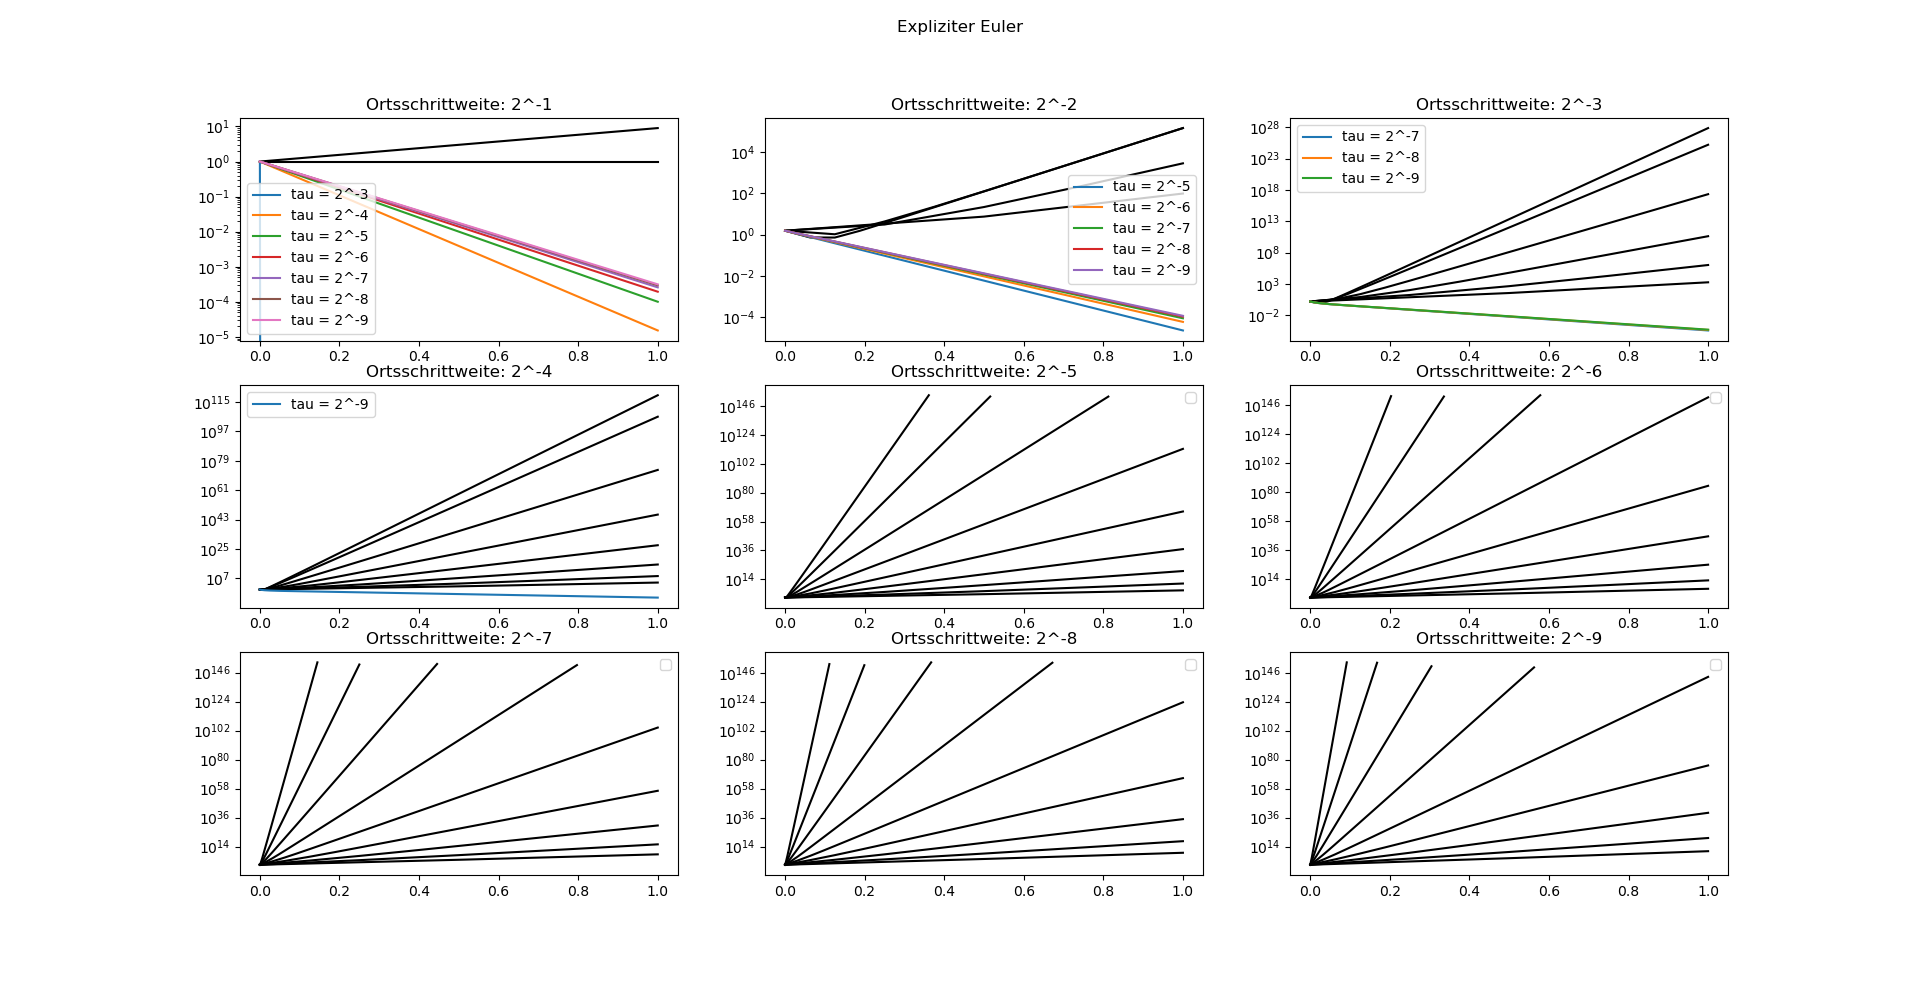
\includegraphics[width=\linewidth]{plot29a.png}
    \caption{Expliziter Euler}
\end{figure}
\FloatBarrier
\item Nun zum impliziten Euler-Verfahren. Wir würden erwarten, dass wir
unabhängig von der Zeitschrittweite exponentiell abfallende Resultate sehen
und die numerischen Tests bestätigen das.
\begin{figure}
    \centering
    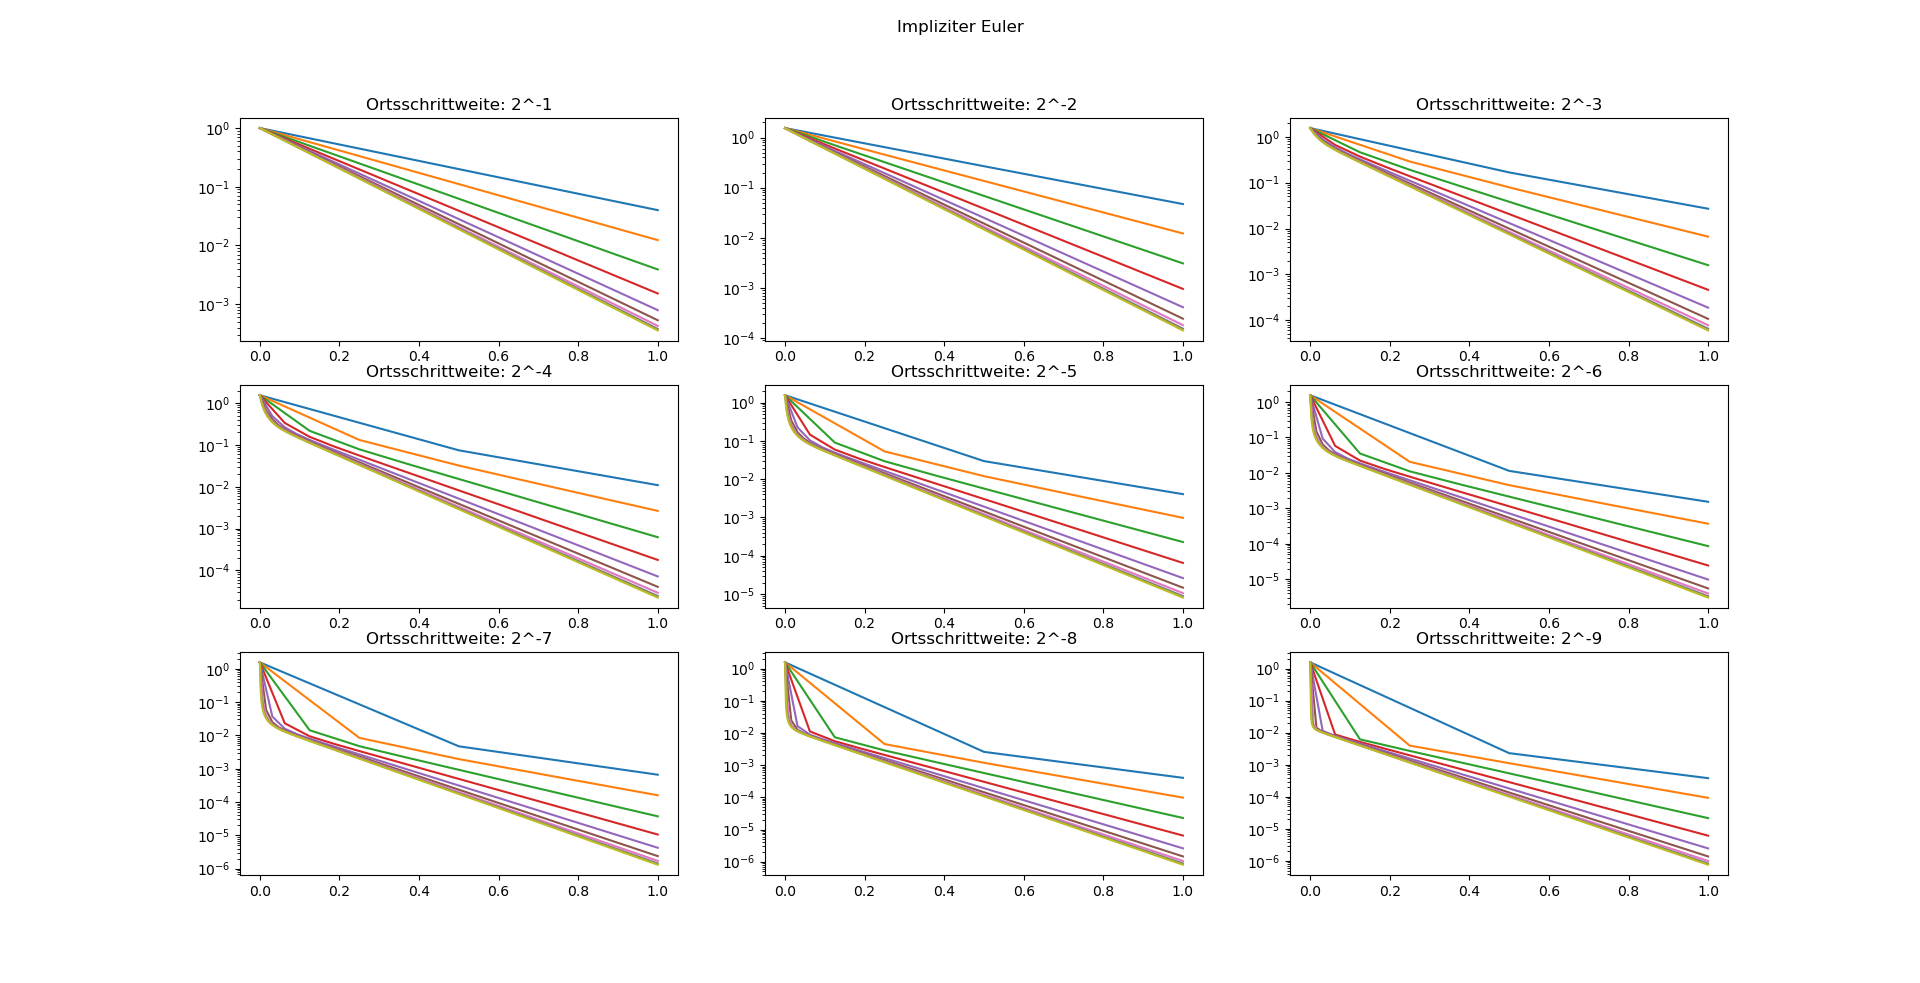
\includegraphics[width=\linewidth]{plot29b.png}
    \caption{Impliziter Euler}
\end{figure}
\FloatBarrier
\end{enumerate}
\end{solution}
